%!TEX root = ../main.tex
% file: assignment2.tex


\graphicspath{{C:/Documents and Settings/amcelhinney/My Documents/GitHub/MCS507ProjectTwo/tex/include/}}

\section{Assignment Three: More Challenging Inputs and Examples} % (fold)
\label{sec: First}


\subsection{The Boston Housing Data Set} % (fold)
\label{sub:methoda}
To provide a more interesting data set to examine the Earth software implementation of the MARS algorithm, we sought assistance from the UCI Machine Learning Repository which publishes numerous data sets for the benefit of researchers. We chose the Boston Housing Data Set, which is a famous data set outlining housing prices in suburban Boston. The data set contains the following variables:

\begin{enumerate}
\item CRIM: per capita crime rate by town
\item ZN: proportion of residential land zoned for lots over 25,000 sq.ft.
\item INDUS: proportion of non-retail business acres per town
\item CHAS: Charles River dummy variable (= 1 if tract bounds river; 0 otherwise)
\item NOX: nitric oxides concentration (parts per 10 million)
\item RM: average number of rooms per dwelling
\item AGE: proportion of owner-occupied units built prior to 1940
\item DIS: weighted distances to five Boston employment centres
\item RAD: index of accessibility to radial highways
\item TAX: full-value property-tax rate per \$10,000
\item PTRATIO: pupil-teacher ratio by town
\item B: $1000(Bk - 0.63)^{2}$ where Bk is the proportion of blacks by town
\item LSTAT: \% lower status of the population
\item MEDV: Median value of owner-occupied homes in \$1000's
\end{enumerate}

This data set was chosen for the following reasons:
\begin{enumerate}
\item The dataset contains categorical, integer and real variables
\item The number of instances ($n=506$) and the number of attributes ($m=14$) is representative of many typical real-world data sets
\item The data set does not contain missing values, which the MARS algorithm does not address in its basic form
\end{enumerate}

To begin the analysis, we first load in the data. Then, to explore the data set, we constructed a function to compute scatter plots of all the data versus the target variable. 
\begin{lstlisting}[caption={Load the Data and Explore},label=2nd,firstnumber=25]
# Bring in the data using the C4.5 format, which brings in the .data file and then the .names file
data = orange.ExampleTable("housing")
print data.domain.attributes

names=str(data.domain).replace('[','').replace(']','').split(',')
# Make Scatterplots of all the variables versus the target variable
def scatterplot(data, data_name, target_var):
    import matplotlib.pyplot as plt
    M = len(data[0])-1
    N=len(data)
    fig = plt.figure()

    y=[float(data[l][target_var]) for l in range(N)]

    for i in range(M):
        ax = fig.add_subplot(int(M/4.)+1,4,i+1)
        py.setp(ax.get_xticklabels(), visible=False)
        x=[float(data[k][i]) for k in range(N)]
        ax.scatter(x,y)
        #ax.set_xlabel(data_name[i],size='10')
        ax.set_title(data_name[i],size='10')
        #ax.set_ylabel(data_name[target_var],size='10')
    return fig
fig = scatterplot(data, names, len(data[0])-1)
\end{lstlisting}

\begin{figure}[H]
    \centering
       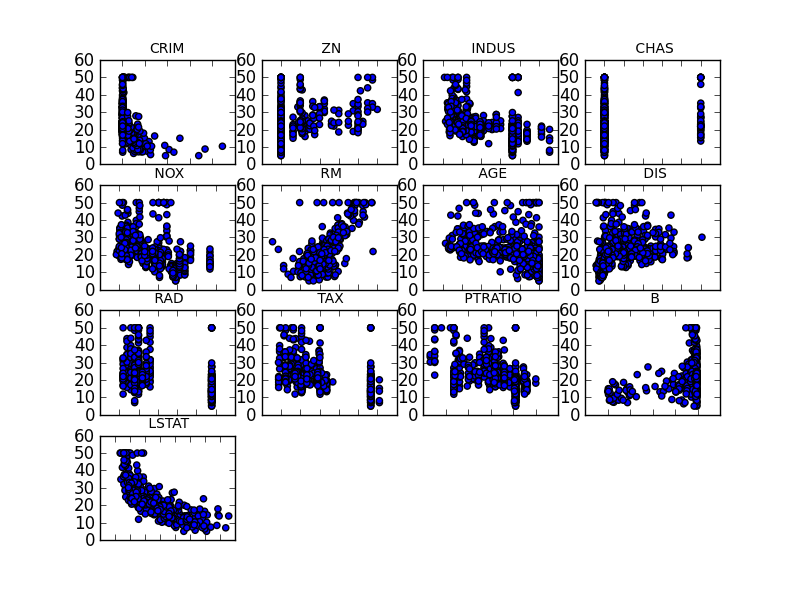
\includegraphics[width=6.5in]{scatter.png}
    \caption{Scatterplot of the Independent Variables vs the Target Variable}
    \label{Example Data}
\end{figure}

\subsection{Fitting the MARS Model} % (fold)

Simiarly to previous examples, the Earth software lets us very quickly view the data, fit the data to the model and then view the model. 
\begin{lstlisting}[caption={Load the Data and Explore},label=2nd,firstnumber=53]
# View the data
for i in range(5):
    print data[i]


earth_predictor = earth.EarthLearner(data)

print earth_predictor
\end{lstlisting}

\begin{equation}
	MEDV =
   33.518
   -0.687 * \max(0, CRIM - 4.422)
   -1.132 * \max(0, 4.422 - CRIM)
\end{equation}
\begin{equation}
\nonumber
+0.560 * \max(0, CRIM - 12.048)-28.029 * \max(0, NOX - 0.488)+7.127 * \max(0, RM - 6.431)
\end{equation}
\begin{equation}
\nonumber
   -0.662 * \max(0, DIS - 2.436)
   +5.010 * \max(0, 2.436 - DIS)
   +0.031 * \max(0, 296.000 - TAX)
\end{equation}
\begin{equation}
\nonumber
-0.637 * \max(0, PTRATIO - 14.700)
   +1.692 * \max(0, 14.700 - PTRATIO)
   -0.355 * \max(0, B - 393.360)
\end{equation}
\begin{equation}
\nonumber
-0.007 * \max(0, 393.360 - B)
   -0.598 * \max(0, LSTAT - 6.120)
\end{equation}
\begin{equation}
\nonumber
   +2.428 * \max(0, 6.120 - LSTAT)
   +0.716 * \max(0, LSTAT - 25.790)
\end{equation}

We then score the data and utilize our previous function to compute the $RSS$ 
\begin{lstlisting}[caption={Compute the RSS},label=2nd,firstnumber=62]
dl=list(data)

# Predict all the data
y_hat=[]
for i in range(0,len(dl)):
    t=earth_predictor.predict(dl[i])
    y_hat.append(t[0])

os.chdir("C:/Documents and Settings/amcelhinney/My Documents/GitHub/MCS507ProjectTwo/src/")
from earth_example import rss
X, Y = data.to_numpy("A/C")

y_1=rss(Y,y_hat)
\end{lstlisting}
The Earth software also allows us to compute and graph the relative importance of each of the variables on the target variable via the \emph{evimp} and \emph{plot\_evimp} methods.
\begin{lstlisting}[caption={Load the Data and Explore},label=2nd,firstnumber=75]
Orange.regression.earth.plot_evimp(earth_predictor.evimp())
\end{lstlisting}
As the graph below shows, the number of rooms the house has (variable $RM$) and the percentage of the population that is lower status in a given area (variable $LSTAT$) are by far the two strongest predictors of housing price. 
\begin{figure}[H]
    \centering
       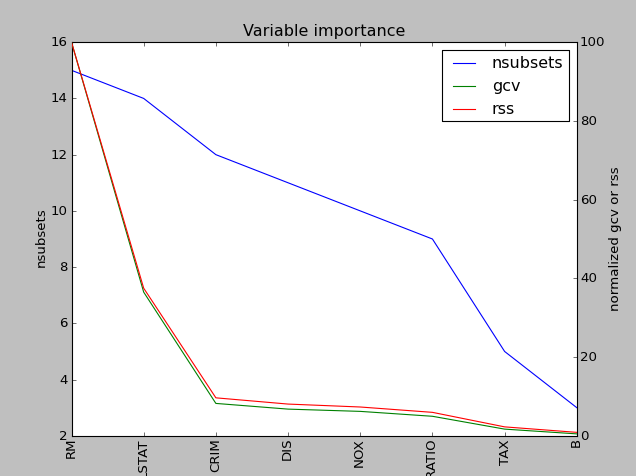
\includegraphics[width=4.in]{variable_importance.png}
    \caption{Relative Importance of the Independent Variables on the Target Variable}
    \label{Example Data}
\end{figure}

Similarly to Assignment 2, we compare the performance of the MARS algorithm versus the traditional least squares regression. However, this time we utilize the \emph{OLS} class from the \emph{SciPy} module. 
\begin{lstlisting}[caption={Fit the OLS Model},label=2nd,firstnumber=77]
# Compute using the standard regression model
import ols
model=ols.ols(Y,X,names[len(names)-1],names[:len(names)-1])
model.summary()
\end{lstlisting}

Unlike the regression fitting packages used in Example 2, the \emph{Ols} class provides us with a full regression output, similar to what one would find in R, SAS, or any other dedicated statistics package.
\begin{figure}[H]
    \centering
       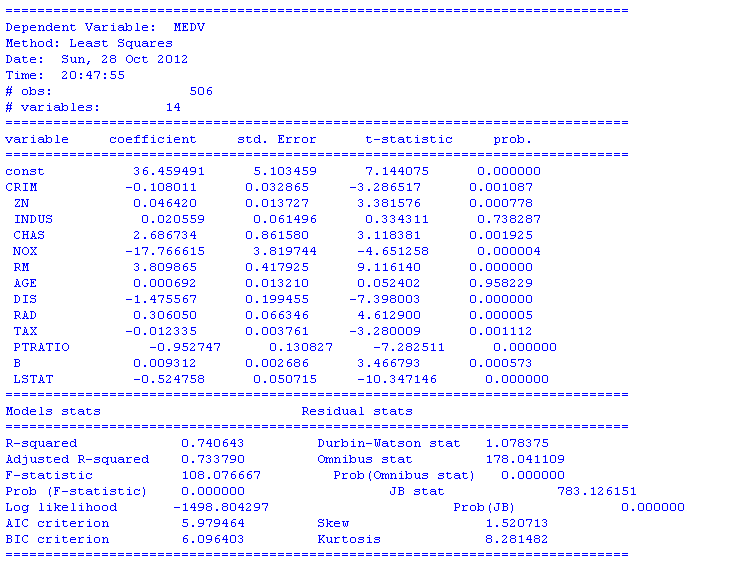
\includegraphics[width=6.5in]{ols_output.png}
    \caption{Output from the \emph{Ols} Class in \emph{SciPy}}
    \label{Example Data}
\end{figure}

Interestingly, the t-statistics for the $RM$ and $LSTAT$ variables are among the largest. This is in alignment with the graph of relative variable importance examined previously. 
\begin{lstlisting}[caption={Calculate the RSS for the OLS Model},label=2nd,firstnumber=83]
# Get the regression coefficients
coeff=model.b
# Score the data
y_hat_ols=[]
for i in range(len(data)):
    y_hat=coeff[0]
    for j in range(len(coeff)-1):
        #print coeff[j+1]
        #print data[i][j]
        y_hat=y_hat+data[i][j]*coeff[j+1]
    y_hat_ols.append(y_hat)
# Compute the RSS
y_2=rss(Y,y_hat_ols)

\end{lstlisting}
Again following the convention from Example 2, we score the data using the OLS Model and compute the $RSS$. 
\begin{table}[H]
\caption{$RSS$ For MARS vs OLS}
\centering
\begin{tabular}{c c}
\hline\hline
Method & $RSS$ \\
\hline
MARS &6311 \\
OLS & 11079 \\
\hline
\end{tabular}
\label{table:nonlin} 
\end{table}
Once again the Earth software shows its utility because the MARS algorithm was better able to predict the target variable as compared to the OLS.
